\part{Mathematik}
\section{Allgemeines}
	Bei Differentialgleichungen\\
	Grad: Höchste vorkommende Potenz\\
	Ordnung: Höchste vorkommende Ableitung\\\\
	Bei üblichen Funktionen deuten diese Bezeichnungen beide auf die höchste Potenz in der Funktion hin.
	
\section{Tensorfelder}
	Als Tensorfeld ist eine Abbildung zu verstehen, die jedem Punkt des Raumes eine Zahl, ein Vektor oder eben ein Tensor bestimmter Stufe zuordnet. So wird zum Beispiel der Spannungszustand eines Materials in jedem Punkt durch einen Spannungstensor zweiter Stufe beschrieben. D.h. im 3-dimensionalen Raum wird die Spannung in einem Punkt durch drei $ 3x3 $ Matrizen festgelegt.
	\begin{figure}[h]
		\centering
		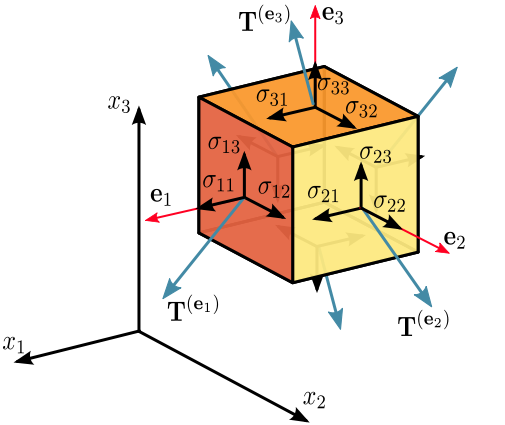
\includegraphics[width=0.4\linewidth]{./pics/ma/spannungstensor}
		\caption{Spannungstensor in der Kontinuumsmechanik}
	\end{figure}
	\leavevmode\\
	
\section{\textcolor{red}{Lineare Algebra}}
\section{\textcolor{red}{Fast Fourier transformation (FFT)}}
	Die FFT ist ein Algorithmus zur effizienten Berechnung der diskreten Fourier-Transformation (DFT). Mit ihr kann ein digitales Signal in seine Frequenzanteile zerlegt und diese dann analysiert werden.
\section{Mathematische Optimierung}
	\subsection{Lineare Optimierung}
		Jedes Problem der linearen Optimierung kann durch eine Zielfunktion
		\[z = \bm{c}^{T}\bm{x}\rightarrow max!\]
		und zugehörige Nebenbedingungen
		\[A\bm{x} \leq \bm{b},\]
		\[\bm{x} \geq 0\]
		formuliert werden.\\\\
		\tab[1cm] \textbf{A} \tab ... \tab $ m\times n- $Matrix mit m Nebenbedingungen und n Variablen inkl. Schlupfvariablen
		\leavevmode \\\\
		Der Lösungsbereich ist immer Polytop (Simplex) und die optimale Lösung befindet sich immer in einer Ecke. Lineare Optimierungsprobleme können deshalb durch Absuchen aller Ecken des zulässigen Bereichs gelöst werden.\\
		\textbf{Satz 1:} Der zulässige Bereich M ist eine konvexe Teilmenge des $ \mathbb{R}^{n} $, d.h. mit zwei Punkten $ \bm{x,y} $ aus M ist auch jede Konvexkombination in M.\\
		\textbf{Satz 2:} Falls der zulässige Bereich M nicht leer und beschränkt ist, so nimmt die Zielfunktion ihr Maximum in mindestens einer Ecke von $ M $ an. \\
		\textbf{Satz 3:} Ein Punkt $ \bm{x} \in M $ ist genau dann eine Ecke von M, wenn die Spaltenvektoren $ a_{j} $ für, welche die zugehörigen Koeffizienten $ x_{j} $ positiv sind, linear unabhängig sind. D.h. für positive $ x_{j} $ müssen die Spalten $ a_{j} $ von A linear unabhängig sein.
		\leavevmode \\\\
		\textbf{Schlupfvariable:} Sie ermöglichen es die Nebenbedingungen statt als Ungleichungen, als Gleichungen anschreiben zu können. Dies beruht auf der Idee, dass die Ungleichung $ x<b $ erfüllt ist, wenn die Gleichung $ x=b-c $ für eine beliebige Zahl $ c>0 $ gilt. Jedes lineare Optimierungsproblem ist in eine solche Normalform überführbar. Die Werte der Schlupfvaraiblen sind für die Lösung des Problems nicht von Interesse.
		\leavevmode \\\\
		\textbf{Erstes Eckenkriterium:} Ist ($ x_{1}, ...,x_{n} $) eine Ecke, dann sind maximal so viele Variablen ungleich von Null, als der Rang der Matrix A (\# NB). Z.b. 3 NB mit zwei Variablen $ x_{1}, x_{2} $ und drei Schlupfvariablen. Eine Ecke kann in diesem Fall maximal drei Variablen ungleich Null besitzen. Sind weniger als drei verschieden von Null, heißt die Ecke entartet. Werden so viele Spalten aus der Matrix A gewählt, dass diese vollen Rang besitzt und damit ein Gleichungssystem angeschrieben, dann ist die Lösung eine zulässige Basislösung wenn alle Variablen größer-gleich Null sind. D.h. wählt man 3 linear unabhängige Spalten von $ \bm{A} $, dann ist dies eine zulässige Basislösung. Andernfalls ist die Basislösung nicht zulässig.\\\\
		Sei $ m $ die Anzahl der Nebenbedingungen (Zeilen von A) und $ n $ die Anzahl der Spalten von A inkl. Schlupfvariablen. Verbleiben nach streichen aller l.a. Spalten noch m=n, dann ist die Lösung eindeutig (1 Punkt mit optimalem Zielfunktionswert). Falls $ \bm{x} $ wenige als $ m $ positive Komponenten hat, so spricht man von einer entartete Ecke.
		\leavevmode \\\\
		\textbf{Zweites Eckenkriterium:} Jede zulässige Basislösung ist eine Ecke. Umgekehrt ist jede nicht entartete Ecke, durch die entsprechenden Spaltennummern eine Basis.
		\leavevmode \\\\
		\textbf{Ein Lösungsalgorithmus:} Man durchlaufe alle Basen aus Spalten der Nebenbedingungsmatrix und berechne zugehörige Basislösungen. Ist diese zulässig, hat man eine Ecke gefunden. Auf diese Weise werden alle Ecken gewonnen. Jene mit dem maximalen Zielfunktionswert ist die optimale Lösung.
		\leavevmode \\\\
		\textbf{Schattenpreise:} Nach einer gefundenen Lösung soll erörtert werden, ob der Zielfunktionswert weiter erhöht werden kann indem die optimale Lösung (Ecke) leicht variiert wird (Beschränkungen in $ \bm{b} $ ändern). Jede Nebenbedingung (i) hat einen Schattenpreis $ \Delta z = \Delta z(i) $, um den sich der Gewinn erhöht, wenn die Beschränkung der entsprechenden Ressource um eine Einheit erhöht wird. Die Beschränkungen werden durch den Vektor $ \bm{b} $ beschrieben.
		\leavevmode \\\\
		\textbf{Sensitivitätsanalyse der Zielfunktion:} Es wird untersucht, in welchem Rahmen die Koeffizienten der Zielfunktion variiert werden können, ohne die gewonnene optimale Lösung zu ändern.
		\leavevmode \\\\
		\textbf{Sensitivitätsanalyse der Einsatzmittelbeschränkung:} Es wird untersucht, in welchem Rahmen die Koeffizienten des Vektors $ \bm{b} $ geändert werden können, sodass die gewählte Basislösung zulässig ($ \bm{x}(i) \geq 0 $) bleibt.
		\leavevmode \\\\
		Das Lösen der Zielfunktion zu einem Optimum wird \textit{primales Problem} genannt. Die Schattenpreise sind die Lösungen des \textit{dualen Problems} oder können auch als sogenannte Lagrangemultiplikatoren erhalten werden.
		\[Z = \bm{b}^{T}\bm{u}\rightarrow min,\]
		\[A^{T}\bm{u} \geq \bm{c},\]
		\[\bm{u} \geq 0\]
		Zielfunktionswerte des primalen und dualen Problems stimmen stets überein. Es gilt
		\[z = \bm{c}^{T}\bm{x} = \bm{b}^{T}\bm{u} = Z.\]
		Daraus folgt, dass die Komponenten von $ \bm{u} $ gerade die Schattenpreise $ \Delta z(i) $ sind. Erhöht man nämlich $ b_{i} $ um eine Einheit, unter Beibehaltung der zulässigen Basis, dann ergibt sich gerade
		\[z_{neu} = \bm{b}^{T}_{neu}\bm{u} = \underbrace{\bm{b}^{T}_{alt}\bm{u}}_{z_{alt}} + \underbrace{1\cdot u_{i}}_{\Delta z}.\]
		\leavevmode \\
		\textbf{Voragangsweise bei Gleichheitsnebenbedingungen:} Falls nicht $ m $ Schlupfvariablen auftreten, müssen stattdessen Hilfsvariablen eingeführt werden um eine Startecke zu finden. In der optimalen Lösungen müssen alle Spalten von Hilfsvariablen mit solchen der ursprünglichen Matrix $ \bm{A} $ getauscht sein, sonst hat das Problem keine Lösung. Man streicht dann die hinteren Spalten, nach Anzahl der eingeführten Hilfsvariablen und erhält eine neue Matrix $ \bm{A} $ mit einer Einheitsmatrix am Anfang. 
		\leavevmode \\\\
		\textbf{Simplexalgorithmus:}
		
		
	\subsection{Ganzzahlige Lineare Optimierung}
		Ein solches Problem wird über Ressourcen $ R_{1}, ...,R_{h} $ und Jobs $ J_{1}, ...,J_{k} $, denen Ressourcen zugeteilt werden können beschrieben. Bekannt seien die Kosten $ c_{ij} $ einer Ressource für einen bestimmten Job. Gesucht ist der optimale, kostengünstigste Zuordnungsplan, bei dem jede Ressource höchstens einen Job und jeder Job von höchstens einer Ressource bearbeitet wird. \\
		Da der Rechenaufwand für das Auffinden aller optimalen Lösungen sehr groß werden kann, wird über das \textit{Branch-and-Bound-Verfahren} ein reduzierter Entscheidungsbaum erstellt.
		\begin{figure}[h]
			\centering
			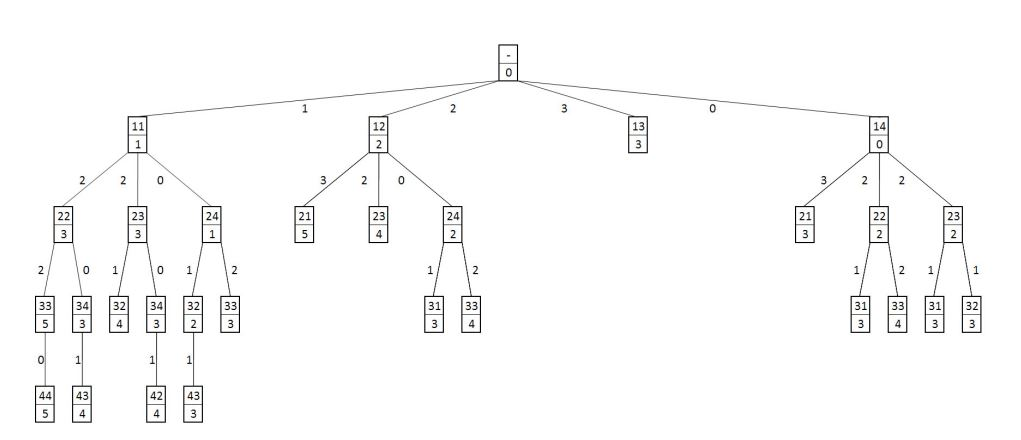
\includegraphics[width=0.7\linewidth]{./pics/ma/bnd} 
			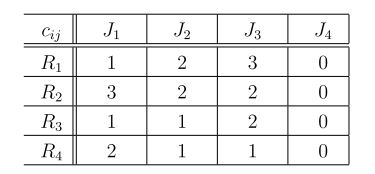
\includegraphics[width=0.29\linewidth]{./pics/ma/bndt}
		\end{figure}
		\leavevmode \\
		Ein Zweig wird terminiert, falls längs diese Zweigs kein niederer Zielfunktionswert erzielt werden kann. Oben im Knoten ist die Indexierung und unten der Zielfunktionswert eingetragen. An den Kanten sind die Kosten aufgetragen.
		\leavevmode \\\\
		\textbf{Rucksackproblem}\\
		Gegeben sind $ n $ Ausrüstungen mit Gewichten $ g_{1}, ...,g_{n} $ und den Werten $ w_{1}, ..., w_{n} $. Gesucht ist die Kombination an Ausrüstung mit dem maximalen Gesamtwert $ W $, deren Gesamtgewicht unterhalb einer vorgeschriebenen Grenze $ G $ ist. Zur Formulierung ob der Gegenstand gewählt wurde, wird $ x_{j} = 1 $ und falls nicht $ x_{j} = 0 $ gesetzt.
		\[W = \sum_{j=1}^{n} w_{j}x_{j}\rightarrow max\]
		\[\sum_{j=1}^{n} g_{j}x_{j} \leq G\]
		Gestartet wird mit der Summe der Werte aller Gegenstände $ W_{O} = \sum_{j=1}^{n} w_{j} $ und einer unteren Gewichtsschranke $ G_{0} = 0 $. Wird ein Gegenstand ausgewählt ($ x_{j} = 1 $), dann wird zur unteren Gewichtsschranke $ G_{U} $ das Gewicht $ g_{j} $ hinzu addiert. Falls der Gegenstand nicht verwendet wird ($ x_{j} = 0 $), dann wird der maximal erreichbare Gesamtwert $ W $ um den Wert $ w_{j} $ verringert. Ein Zweig wird terminiert, wenn die untere Gewichtsschranke die vorgegebene Gewichtsschranke überschreitet $ G_{U} > G $ oder wenn eine neue obere Wertschranke $ W_{O} $ kleiner wird als der aktuelle Gesamtwert $ W_{A} $.
		\begin{figure}[h]
			\centering
			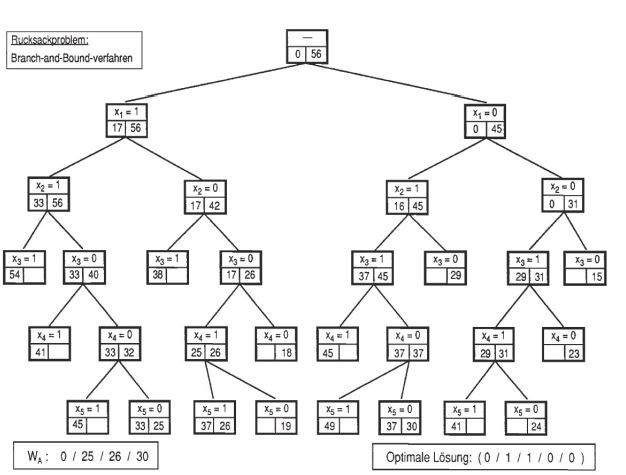
\includegraphics[width=0.6\linewidth]{./pics/ma/rucksack}
			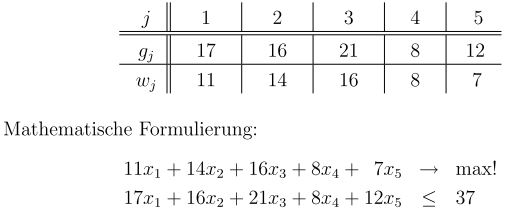
\includegraphics[width=0.39\linewidth]{./pics/ma/rucksackt}
		\end{figure}
		\leavevmode \\\\
		\textbf{Das Allgemeine Problem, Dakin-Verfahren}\\
		Das allgemeine ganzzahlige Optimierungsproblem hat die Form
		\[W = \sum_{j=1}^{n}c_{j}x_{j} \rightarrow max\]
		\[\sum_{j=1}^{n} a_{ij}x_{j} \leq b_{j}\]
		\[x_{j} \geq 0,\text{ } und\text{ } ganzzahlig.\]
		Das Problem wird in mehrere Teilprobleme aufgespalten. Als erstes wird die Ganzzahligkeitsanforderung weggelassen und eine möglicherweise nichtganzzahlige Ecke aus den Nebenbedingungen berechnet. Ebenso der zugehörige Zielfunktionswert, der ebenfalls nichtganzzahlig sein kann.\\
		Diese Lösung wird aufgespalten, indem man die erste nichtganzzahlige Variable nimmt und die größte ganzzahlige Zahl $ x_{j} $ nennt. Z.b. von 3.75 $ \rightarrow x_{j} = 3 $. Über die jeweilige NB werden dann die restlichen Variablen berechnet. Sind alle Variablen ganzzahlig, wird terminiert. Sind jedoch noch nicht alle Variablen ganzzahlig, wird weiter aufgespalten. Man nimmt die nächste nichtganzzahlige Variable und rundet diese wieder einmal \textit{floor} und \textit{ceil}. Z.b. aus 1.2 $ \rightarrow $ 1 und 2. Falls die Variablen die zugehörige NB verletzen, wird terminiert. Falls das Wählen der zweiten Variable zur Ganzzahl die erste Varaible wieder nichtganzzahlig macht, wird erneut aufgespalten. Dies wird solange iteriert bis alle Zweige terminiert sind. Eine weitere Terminierungsbedingung ist, wenn eine nichtganzzahlige Lösung vorliegt und der zugehörige Zielfunktionswert kleiner als größte bereits bekannte Zielfunktionswert einer zulässigen Lösung ist.
		\begin{figure}[h]
			\centering
			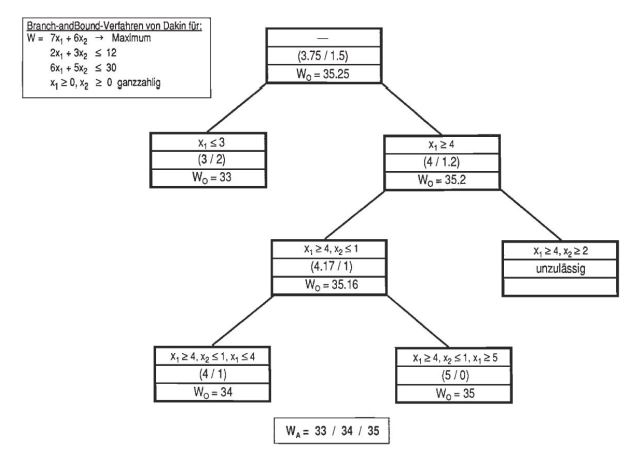
\includegraphics[width=0.7\linewidth]{./pics/ma/dak}
			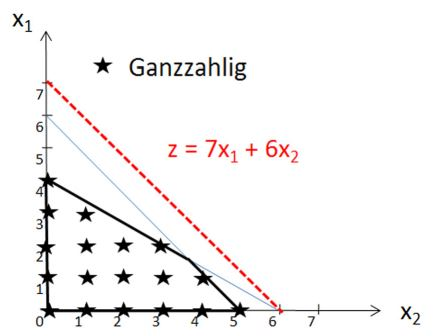
\includegraphics[width=0.29\linewidth]{./pics/ma/dakd}
		\end{figure}
		\leavevmode \\\\
		\textbf{Das Reihenfolgeproblem, Johnson-Algorithmus (\textit{greedy-algorithm})}\\
		Es seien $ n $ Jobs gegeben die hintereinander auf Maschine $ M_{1} $ und dann auf $ M_{2} $ erledigt werden müssen. Die Bearbeitungszeit des Jobs $ j $ sei auf $ M_{1} $ sei $ a_{j} $ und auf $ M_{2} $, $ b_{j} $. Gesucht ist der optimale Belegungsplan, der die optimale Reihenfolge mit der kürzesten benötigten Gesamtzeit aufweist (äquivalent: kürzeste Standzeiten der Maschinen).\\\\
		Für zwei Maschinen liefert der Johnson-Algorithmus eine exakte Lösung. Bei mehreren Maschinen bzw. komplizierteren Arbeitsabläufen kann das Problem als allgemeine ganzzahlige Optimierungsaufgabe gestellt  und mit dem Dakin-Verfahren gelöst werden.\\\\
		Man suche $ min(a_{1}, ...,a_{n},b_{1}, ...,b_{n}) $. Ist der kürzeste Arbeitsschritt $ a_{j} $, wird der Job $ j $ als Erstes abgearbeitet. Ist der kürzeste Arbeitsschritt $ b_{j} $, dann wird der Job $ j $ als letztes abgeschlossen. Dann wird Job $ j $ gestrichen und der Vorgang beginnt von vorne, bis man die optimale Reihenfolge der Jobs gefunden hat.
	
	\subsection{Globale Optimierung}
		Die allgemeine Aufgabe besteht darin, eine Funktion $ f $ über eine abgeschlossene Teilmenge $ D $ zu minimieren.
		\[f(x) \rightarrow min, \quad x\in D\]
		$ D $ wird durch Nebenbedingungen in Form von Gleichungen und Ungleichungen gegeben. Maximierungsaufgabe ist wegen $ max(f) = -min(-f) $ ebenfalls abgedeckt. Falls die Gleichungen differenzierbar sind, bietet sich die Methode der \textit{Lagrangemultiplikatoren} an.
		\leavevmode \\\\
		\textbf{Lagrangemultiplikatoren, NB als Gleichungen}\\
		Für eine gegebene differenzierbare Funktion $ f $ soll die Minimierungsaufgabe
		\[f(x) \rightarrow min\]
		unter den Nebenbedingungen
		\[g_{1}(x)=0, ...,g_{k}(x)=0\]
		gelöst werden, wobei die NB differenzierbar und ihre Gradienten
		\[\nabla g_{1}(x), ...,\nabla g_{k}(x)\]
		als linear unabhängig vorausgesetzt werden. Die \textit{Lagrangemultiplikatorregel} wird wie folgt angewendet.\\\\
		\textit{1. Schritt:} Man bilde die Hilfsfunktion in n+k Variablen $ x_{1}, ...,x_{n},u_{i}, ...,u_{k} $
		\[L(\bm{x},\bm{u}) = f(\bm{x}) + \bm{u}^{T}\bm{g}(\bm{x})\]
		und berechne die Gradienten der Hilfsfunktion.\\\\
		\textit{2. Schritt:} Man bestimmte die stationären Punkte der Lagrangefunktion. Das sind die Lösungen des Gleichungssystems 
		\[\nabla L(x_{1}, ...,x_{n},u_{i}, ...,u_{k}) = \bm{0}.\]
		Das heißt,
		\[\frac{\partial}{\partial x_{i}} L = \frac{\partial}{\partial x_{i}}f(\bm{x}) + u_{1}\frac{\partial}{\partial x_{i}}g_{1(x)}+ ... + u_{k}\frac{\partial}{\partial x_{i}}g_{k}(\bm{x})\]
		\[\frac{\partial}{\partial u_{j}}L = g_{j}(\bm{x}) = \bm{0}\]
		für $ i = 1, ...,n $ und $ j = 1, ...,k $\\\\
		\textit{3. Schritt:} Die Maxima und Minima sind unter den Lösungen ($ x_{1}, ..., x_{n} $) zu finden.
		\leavevmode \\\\
		\textbf{Lagrangemultiplikatoren, NB als Ungleichungen}\\
		Liegen die Nebenbedingungen als Ungleichungen vor,
		\[f(x) \rightarrow min\]
		\[\bm{g(x)} \leq \bm{0}, \quad \bm{x} \geq \bm{0} \]
		so bildet man ebenfalls die Lagrangefunktion
		\[L(\bm{x},\bm{u}) = f(\bm{x}) + \bm{u}^{T}\bm{g}(\bm{x}).\]
		Anstelle des Aufsuchens der stationären Punkte der Lagrangefunktion sind jetzt die Sattelpunkte zu ermitteln. Ein Paar ($ \bm{x,u} $) mit $ \bm{x} \geq \bm{0}, \quad \bm{u} \geq \bm{0} $ heißt Sattelpunkt, falls
		\[L(x,v) \leq L(x,u) \leq L(y,u)\]
		für alle $ (\bm{y,v}) $ mit $ \bm{y} \geq \bm{0}, $  $ \bm{v} \geq \bm{0} $ erfüllt ist. Das heißt ($ \bm{x,u} $) ist ein Sattelpunkt wenn der Funktionswert beim Verlassen des Punktes in \textit{v-Richtung} abnimmt ($ L(x,v) $) und in \textit{y-Richtung} zunimmt ($ L(y,u) $).
		\subsubsection{Quadratische Optimierung}
			Das quadratische Standardproblem ist
			\[f(\bm{x}) = \bm{x}^{T}\bm{Ax} - \bm{b}^{T}\bm{x}\]
			mit einer symmetrischen und positiv definiten Matrix $ \bm{A} $. Das Lösen des linearen Gleichungssystems $ \bm{Ax} = \bm{b} $ ist äquivalent und führt zum selben Ergebnis. Denn der Gradient ist
			\[\nabla f(\bm{x}) = \bm{Ax}-\bm{b}.\]
			\textit{Vorkonditionierung:} Eine Matrix $ \bm{B} $ zur Vorkonditionierung dient dazu die Kondition, also die Abhängigkeit der Lösung von den Eingangsdaten, zu verringern.\\\\
			Eine Iteration kann dann folgendermaßen geschrieben werden, wobei $ \alpha $ die Distanz in die Abstiegsrichtung $ \bm{s}_{k} $ bis zur nächsten Iteration $ \bm{x}_{k+1} $ beschreibt.
			\[\bm{x}_{k+1} = \bm{x}_{k} + \alpha \bm{s}_{k}, \qquad \bm{Bs}_{k} = \bm{b} - \bm{Ax}_{k} \quad \Rightarrow \quad \bm{s}_{k} = -\bm{B}^{-1}\nabla f(\bm{x}_{k}) \]
			Bei der \textit{konjugierten Gradienten Methode} wird die Abstiegsrichtung $ \bm{p}_{k} $ nochmals mit dem Relaxationsfaktor $ \beta_{k} $ korrigiert, um ein Optimum in weniger Iterationen zu finden.
			\[\bm{p}_{k} = \bm{s}_{k} + \beta_{k}\bm{p}_{k-1} \]
			Sobald der Betrag des Gradienten eine gewisse Toleranz unterschreitet werden die Verfahren abgebrochen.
		\subsubsection{Lineare kleinste Fehlerquadrate}
			Das Problem überbestimmter linearer Systeme und die Minimierung der Summe der Fehlerquadrate ist
			\[f(\bm{x}) = ||\bm{Ax}-\bm{b}||^{2} \rightarrow min.\]
			Man kann auch
			\[f(\bm{x}) = (\bm{Ax}-\bm{b})^{T}(\bm{Ax}-\bm{b}) = \bm{x^{T}A^{T}Ax} - 2\bm{x^{T}A^{T}b} + \bm{b^{T}b} \]
			schreiben. Über die partiellen Ableitungen, den Gradienten 
			\[\nabla f(\bm{x}) = 2\bm{A^{T}Ax} - 2\bm{A^{T}b}\]
			und der Bedingung, dass dieser zu Null wird, können die gesuchten Parameter $ \bm{x} $ über das lineare Gleichungssystem
			\[\bm{A}^{T}\bm{Ax} = \bm{A}^{T}\bm{b}\]
			berechnet werden. Die Bedingung $ \nabla f(\bm{x}) = \bm{0} $ folgt aus der Forderung das Fehlerquadrat zu minimieren. Da das Fehlerquadrat in jedem Punkt konstant ist, ergibt sich in den partiellen Ableitungen jedes Punktes, dieser Wert zu Null.
		\subsubsection{Nichtlineare kleinste Fehlerquadrate}
			Eine Idee ist dieses nichtlineare Problem als eine Abfolge von linearen kleinsten Fehlerquadraten iterativ zu Lösen. Die nichtlineare Funktion $ \bm{F(x)} $ wird über die Taylor-Entwicklung durch quadratische Funktionen angenähert, die wiederum zum Lösen des linearen Gleichungssystems $ \bm{Ax} - \bm{b} $ äquivalent sind (\textit{Gauss-Netwon Verfahren}). Der Vorteil ist, dass die oft schwierig zu berechnenden zweiten Ableitungen nicht benötigt werden.
			\[\bm{F(x)} \approx \bm{F(x^{k})} + \bm{J}_{F}(\bm{x}^{k})(\bm{x} - \bm{x}^{k}) \]
			Der nächste Iterationsschritt wird durch Lösung des Minimierungsproblems
			\[f(\bm{x}) = ||\bm{F(x^{k})} + \bm{J}_{F}(\bm{x}^{k})(\bm{x} - \bm{x}^{k})||^{2} \rightarrow min\]
			gewonnen. Mit $ \bm{A} = \bm{J}_{F}(\bm{x}^{k}), $ $ \bm{s}^{k} = \bm{x-x}^{k} $ und $ \bm{b} = -\bm{F(x^{k})} $ erhalten wir das Problem der linearen kleinsten Fehlerquadrate
			\[||\bm{As}^{k} - \bm{b}||^{2}\rightarrow min \]
			Verbesserte Varianten beheben das Problem, dass sich die Summe der Fehlerquadrate nicht mit jeder Iteration verringern. Das Problem liegt bei $ \alpha $ der in Abstiegsrichtung ein zu großes Inkrement verweist. Dafür ist ein \textit{line search} notwendig, das die Zielfunktion in Abstiegsrichtung minimiert. Auch bei der \textit{trust region Gauss-Newton} Methode geht es darum, die \textit{sufficient decrease condition} zu erfüllen. Durch das folglich reduzierte auswerten von Funktionswerten wird der Algorithmus effizienter und benötigt weniger Iterationsschritte.
		\subsubsection{Ableitungsfreie Methoden}
			\textbf{Koordinatensuch-Methoden}\\
			Sie basieren auf der Suche von Funktionswerten anhand eines Rasters auf dem die Zielfunktion ausgewertet wird. Schritt für Schritt bewegt man sich mit dem Raster in Richtung absteigender Zielfunktionswerte. Wird kein kleinerer Zielfunktionswert auf dem Raster gefunden, wird das Raster verfeinert. Um die Wahrscheinlichkeit eines Verfangens in lokalen Minimas zu verringern werden zufällig gewählte Startwerte durchprobiert und der Algorithmus durchgeführt. Man wählt dann denn kleinsten Zielfunktionswert aus allen \textit{runs}.
			\leavevmode\\\\
			\textbf{Downhill-Simplex-Methode}\\
			Die Startkonfiguration ist eine Selektion aus $ n+1 $ Punkten $ \mathbb{R}^{n} $. \\
			Schritt1: Diese Punkte sind nach ihren Funktionswerten (beste $ \rightarrow $ schlechtester) geordnet. In einer Iteration wird der schlechteste Punkt durch Reflexion, Expansion oder Kontraktion ausgetauscht.\\
			Schritt 2: Berechne den Mittelpunkt des Dreiecks.\\
			Schritt 3: Zuerst wird der reflektierte Punkt mit dem schlechtesten Funktionswert berechnet. Ist der reflektierte Punkt besser als der Beste, dann berechne den expandierten Punkt (Schritt 4) und ersetzte den schlechtesten durch den besseren (Reflexion oder Expansion). Zurück zu Schritt 1. Ist der reflektierte Punkt nur besser als der zweitschlechteste, dann ersetzte den schlechtesten durch den Reflektierten. Zurück zu Schritt 1.\\
			Schritt 5: Falls der reflektierte Punkt nicht besser als der Zweitschlechteste (Mittlere) ist, dann berechne den kontrahierten Punkt. Falls dieser besser als der Reflektierte ist, dann ersetzte den schlechtesten durch diesen. Zurück zu Schritt 1.\\
			Schritt 6: Wird durch Reflexion, Expansion oder Kontraktion kein besserer Funktionswert mehr erreicht, kann durch Reduktion aller Punkte zum besten hin, der Zielfunktionswert noch verbessert werden.
			\leavevmode\\\\
			\textbf{Simmulierte Abkühlung}\\
			Grundidee ist die Nachbildung eines Abkühlungsprozesses, etwa beim Glühen in der Werkstoffkunde. Nach Erhitzen eines Metalls sorgt die langsame Abkühlung dafür, dass die Atome ausreichend Zeit haben, sich zu ordnen und stabile Kristalle zu bilden. Dadurch wird ein energiearmer Zustand nahe am Optimum erreicht. \\
			Es wird ein Startwert $ \bm{x} $ und eine Temperaturfolge die gegen Null fällt gewählt. Der Wert wird mit einem Nachbarspunkt $ \bm{y} $ verglichen $ \Delta f = f(\bm{x}_{0})-f(\bm{y}) $.\\
			Falls $ \Delta f > 0 $ dann wird $ \bm{x}_{1}=\bm{y} $ gewählt.\\
			Falls $ \Delta f \leq 0 $ dann wird nur mit einer Wahrscheinlichkeit der Punkt $ \bm{x}_{1}=\bm{y} $ übernommen und mit einer Gegenwahrscheinlichkeit wird der Schritt erneut mit einem anderen Nachbarspunkt ausgeführt.\\
			Dies wird für jeden Temperaturschritt durchgeführt.\\
			\textit{Verdeutlichung: } Angenommen, man sucht in einer zweidimensionalen Landschaft den (global) tiefsten Punkt. Die Landschaft selbst besteht aus vielen unterschiedlich tiefen Dellen. Die einfache Suchstrategie (suche den nächsten tiefsten Punkt) entspricht dem Verhalten einer Kugel, welche in dieser Landschaft ausgesetzt wird. Sie rollt zum nächsten lokalen Minimum und bleibt dort. Bei der simulierten Abkühlung wird der Kugel immer wieder ein Stoß versetzt, der mit zunehmender „Abkühlung“ schwächer wird. Dieser ist idealerweise stark genug, um die Kugel aus einer flachen Delle (lokales Minimum) zu entfernen, reicht aber nicht aus, um aus dem globalen Minimum zu fliehen.
			\leavevmode\\\\
			\textbf{Surrogate-Modelling}\\
			Es werden einfachere Modelle verwendet, die die Optimierungsfunktion annähern. Es wird dann diese Näherung optimiert.\\
			Beispielsweise kann eine echte Optimierungsfunktion durch kubische Splines interpoliert werden. Man kann dann für jeden lokalen Spline das Optimum berechnen und erhält somit auch das genäherte Optimum der Zielfunktion.
			\leavevmode\\\\
			\textbf{Genetische Algorithmen}\\
			Diese Algorithmen ahmen natürliche Selektion nach.  
			\begin{itemize}
				\item Es wird mit einem Set von \textit{Parents} gestartet. $ \bm{P} = [x_{1}, ..., x_{n}] $
				\item Für jeden Parent wird eine Fitness berechnet. $ F(x_{1}), ..., F(x_{n}) $
				\item Bis ein Abbruckkriterium erfüllt ist
				\begin{itemize}
					\item Selektion und Rekombination von Individuen anhand von Fitnesswerten 
					\item Mutation
					\item Fitnessevaluation
					\item Selektion einer neuen Generation
				\end{itemize}
			\end{itemize}
			\leavevmode
			\textbf{Partikelschwarm-Optimierung}\\
			Als Partikelschwarmoptimierung (PSO) wird ein naturanaloges Optimierungsverfahren bezeichnet, das nach dem Vorbild des biologischen Schwarmverhaltens eine Lösung für ein Optimierungsproblem sucht. Analog zum natürlichen Phänomen wird eine Population von Lösungskandidaten durch den Suchraum bewegt, um eine gute Lösung für das Problem zu erhalten. In jedem Rechenschritt wird dazu die Position jedes Individuums und der zugehörige Funktionswert neu berechnet. Beim Schwarm haben die Nachbarn Einfluss auf ein Individuum. Voraussetzung ist ebenfalls das der Schwarm zusammenhält.
			\leavevmode\\\\
			\textbf{Neuronale Netzwerke}\\
			Ein neuronales Netz besteht aus einer Eingangsschicht, einer oder mehrerer Schichten aus künstlichen Neuronen (Übertragungsfunktionen) und einer Ausgangsschicht. Nach der Konstruktion eines Netzes folgt die Trainingsphase. Beim Lernen werden neue Verbindungen gesetzt, gelöscht, die Gewichtung verändert, Schwellwerte angepasst oder ganze Neuronen hinzugefügt oder gelöscht. Jedes Neuron hat demnach einen Threshold ab dem es aktiviert wird und ein Gewicht mit dem der Eingang, dem Ausgang übergeben wird.
			
	\subsection{Konvexe Optimierung}
		Der zentrale Standardfall der nichtlinearen Optimierung ist die konvexe Optimierung, bei der die Funktion $ f $ und $ g_{i} $ als konvex vorausgesetzt werden. $ f $ heißt \textit{konvex}, wenn der Graph unterhalb der Verbindungsgeraden, zweier auf der Funktion liegende Punkte, verläuft.
		\begin{figure}[h]
			\centering
			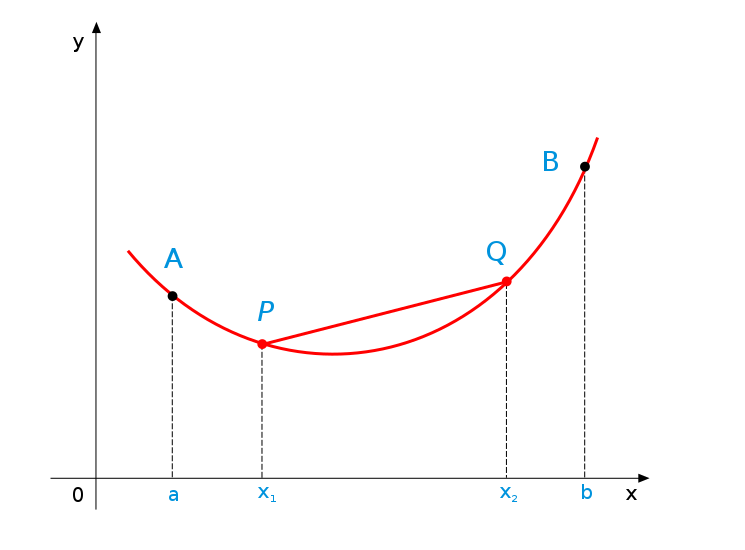
\includegraphics[width=0.3\linewidth]{./pics/ma/konvex}
		\end{figure}
		\[f(\mu \bm{P} + (1-\mu)\bm{Q}) \leq \mu f(\bm{P}) + (1-\mu)f(\bm{Q}), \quad 0\leq \mu \leq 1  \]
		\leavevmode \\
		Die NB sind Ungleichungen. Es kann jedoch aus $ g_{j} \leq 0 $ und $ -g_{j} \leq 0 $, eine Gleichheitsnebenbedingung $ g_{j} = 0 $ gebildet werden. Falls die definierende Ungleichung strikt ($ < $ statt $ \leq $) ist, so heißt die Funktion \textit{streng konvex}. Eine partiell differenzierbare Funktion ist genau dann konvex, wenn für alle $ \bm{x,y} $ gilt
		\[f(\bm{y}) \geq f(\bm{x}) + (\bm{y}-\bm{x})^{T}\nabla f(\bm{x}).\]
		Das heißt, wenn ihr Graph für jeden Punkt oberhalb der zugehörigen Tangente verläuft. Für das Lösen eines konvexen Optimierungsproblems gehen wir davon aus, dass alle beteiligten Funktionen $ f $ und $ g_{i} $ konvex sind. Die NB können in einem Vektor $ \bm{g(x)} = [g_{1}(\bm{x}), ..., g_{m}(\bm{x})]^{T} $ zusammengefasst werden und führen den konvexen zulässigen Bereich ein, der durch die NB definiert wird.
		\[M = \{\bm{x} \in \mathbb{R}^{n}: \bm{g(x)} \leq \bm{0}, \bm{x} \geq \bm{0}\}\]
		Zur Lösung des Optimierungsproblems wird die \textit{Lagrangefunktion} mit den \textit{Lagrangemultiplikatoren} $ u_{j} $ gebildet
		\[L(\bm{x},\bm{u}) = f(\bm{x}) + \bm{u}^{T}\bm{g}(\bm{x}) = f(\bm{x}) + \sum_{j=1}^{m}u_{j}g_{j}.\]
		\textbf{Satz:} Falls ein Paar $ (\bm{x,u}) $ ein Sattelpunkt der \textit{Lagrangefunktion} $ L $ ist, so ist $ \bm{x} $ die Lösung der Minimierungsaufgabe.\\\\
		\textit{Slater-Bedingung:} Falls der zulässige Bereich $ M $ innere Punkte $ \bm{x'} $ besitzt, d.h. falls es mindestens ein $ \bm{x'} \geq \bm{0}$ gibt für den $ \bm{g(x')} < \bm{0} $ gilt. \\\\
		\textbf{Theorem von Kuhn-Tucker:} Falls $ M $ die \textit{Slater-Bedingung} erfüllt, dann ist $ \bm{x} \geq \bm{0} $ genau dann eine Lösung des Minimierungsproblems, wenn es ein $ \bm{u} \geq \bm{0} $ gibt und das Paar $ (\bm{x,u}) $ ein Sattelpunkt von $ L $ ist.
		\[\frac{\partial L}{\partial \bm{x}} \geq 0, \quad \bm{x}^{T}\partial_{x} L(\bm{x,u}) = 0, \quad \bm{x} \geq \bm{0} \]
		\[\frac{\partial L}{\partial \bm{u}} \leq 0, \quad \bm{u}^{T}\partial_{u} L(\bm{x,u}) = 0,  \quad \bm{u} \geq \bm{0}\]
		Man muss also für eine Funktion $ f $ und die NB in Form von Ungleichungen prüfen ob die obigen Kuhn-Tucker Bedingungen, sowie $ \bm{x} \geq \bm{0} $, $ \bm{u} \geq \bm{0} $ erfüllt sind. Sind die Kuhn-Tucker Beidngungen erfüllt, dann ist $ (\bm{x,u}) $ ein Sattelpunkt und $ \bm{x} $ somit eine Lösung des Minimierungsproblems.
		\leavevmode \\\\
		\textbf{Quadratische Optimierung mit Kuhn-Tucker}\\
		Das Standardproblem der quadratischen Optimierung mit linearen NB ist
		\[f(\bm{x}) = \bm{x}^{T}\bm{Cx} + \bm{c}^{T}\bm{x} \rightarrow min\]
		\[\bm{Ax} \leq \bm{b}, \quad \bm{x} \geq \bm{0}.\]
		Mit positiv semidefiniter ($ \bm{x}^{T}\bm{Cx} \geq 0 $) Matrix $ \bm{C} $. Die \textit{Lagrangefunktion} ist dann
		\[L(\bm{x,u}) = \bm{x}^{T}\bm{Cx} + \bm{c}^{T}\bm{x} + \bm{u}^{T}(\bm{Ax} - \bm{b}).\]
		Die zugehörigen Gradienten werden als $ \bm{v} $ und $ \bm{-y} $ definiert
		\[\partial_{x} L(\bm{x,u}) = 2\bm{Cx} + c + \bm{A}^{T}\bm{u} =: \bm{v},\]
		\[\partial_{u} L(\bm{x,u}) = \bm{Ax} - \bm{b} =: \bm{-y}\]
		Die Sattelpunktbedingungen werden dann über die Kuhn-Tucker Bedingungen als
		\[\bm{v} \geq \bm{0}, \quad \bm{x}^{T}\bm{v} = 0,\]
		\[\bm{y} \geq \bm{0}, \quad \bm{u}^{T}\bm{y} = 0,\]
		formuliert.
	\subsection{Variationsrechnung}
		Ein Funktional ist eine Funktion, die anderen Funktionen Zahlen zuordnet. Es ist also eine Abbildung $ \phi : M \rightarrow \mathbb{R} $ von einer Funktionenmenge in die reellen Zahlen. Ein Funktional ordnet also jeder Funktion $ u \in M $ eine Zahl $ \phi(u) $ zu. Ziel der Variationsrechnung ist die Minimierung solcher Funktionale.\\\\
		\textit{Fundamentallemma der Variationsrechnung:} Ist $ f $ eine stetige Funktion und $ \int_{x_{0}}^{x_{1}}f(x)v(x)dx = 0 $ für alle stetigen Funktionen $ v $ und auch $ v(x_{0}) = v(x_{1}) = 0 $, dann ist auch $ f(x) = 0 $ für alle $ x \in [x_{1},x_{1}] $.\\\\
		Die \textit{erste Variation} ist eine verallgemeinerte Richtungsableitung eines Funktionals $ \phi : M \rightarrow \mathbb{R} $. Eine Änderung $ v \in V $ ($ V $ sei Funktionenraum) heißt zulässig, wenn $ u + \tau v $ ebenfalls in $ M $ liegt. Für alle $ \tau $ auf einem Intervall [$ -\tau_{0},\tau_{0} $].
		\[\delta \Phi(u)[v] = \frac{d}{d\tau}\Phi(u + \tau v)\bigg|_{\tau=0}\]
		\subsection{\textcolor{red}{Deterministische Optimierungsverfahen}}
			Dia Aufzählung unter deam nur als allgemein Info ganz oba ane.	
			\subsubsection{\textcolor{red}{Nichtlineare Optimierung ohne Nebenbedingungen}}
				\paragraph{Klassische Gradientenverfahren}
				\paragraph{Konjugierte Gradientenverfahren}
					Algorithmen zum finden eines Minimums welche den Gradienten benutzen, "`wandern"' stets in Richtung des steilsten Abstiegs. Der konjugierte Gradient stellt dabei eine effizientere Methode dar, welcher eine Art verbesserte Richtung benutzt.
					Mit dem Verfahren des konjugierten Gradienten, soll das lineare Gleichungssystem $A x=b$ gelöst werden. Die Systemmatrix $A$ ist dabei symmetrisch und positiv definit. Zum lösen gilt es die die Kostenfunktion 
					\[ F(x)=\frac{1}{2}x^T A x  - x^T b\]
					zu minimieren.	
					Das Verfahren soll im folgenden beschrieben werden. Der Startvektor $x_0$ ist dabei beliebig zu wählen. Mit diesem wird der erste Residuenvektor $r_0$ und der erste Korrekturvektor $p_0$ berechnet:
					\[ x_0; \qquad r_0=b-A x_0; \qquad p_0=r_0\] 
					Die folgenden Schritte $i$ werden iterativ berechnet. Der neue Vektor $x_{i+1}$ wird durch den alten Vektor $x_i$ in die Richtung von $p_i$ bestimmt. Die Schrittlänge wird dabei durch den Faktor $\lambda_i$ festgelegt:
					\[ \lambda_i=\frac{r_i^T p_i}{p_i^T A p_i}; \qquad x_{i+1}=x_i + \lambda_i p_i\] 
					Für den nächsten Iterationsschritt wird nun noch ein neuer Residuenvektor $r_{i+1}$ und ein neuer Korrekturvektor $p_{i+1}$ berechnet:
					\[ r_{i+1}=r_i - \lambda_i A p_i; \qquad p_{i+1}=r_{i+1}+\frac{r_{i+1}^T r_{i+1}}{r_i^T r_i} p_i\]
					Das Verfahren konvergiert, abgesehen von Rundungsfehler, nach n Iterationsschritten, wobei n die Größe der quadratischen Matrix $A\in \mathbb{R} ^{n x n}$ ist. 
					Anschaulich formuliert ist die Richtung des neuen Korrekturvektor eine verbesserte Richtung des alten Residuenvektor und zeigt somit besser in Richtung des gesuchten Ziels.
					\begin{figure}[h]
						\centering
						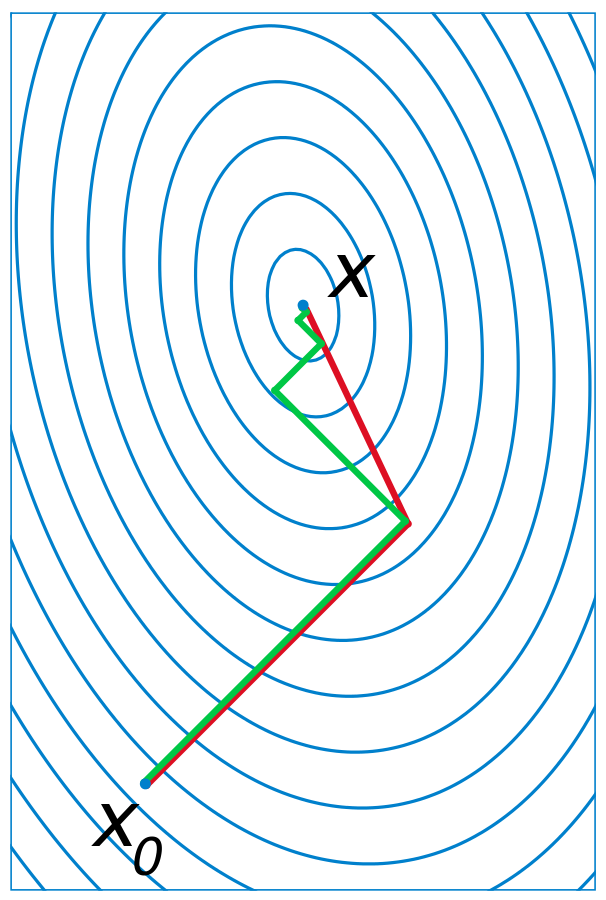
\includegraphics[width=0.3\linewidth]{./pics/ma/konjug.png}
						\caption{Grün: Gradient, Rot: Konjugierter Gradient}
						\label{}
					\end{figure}
					In der Abbildung ist zu erkennen, dass der "`rote"' Weg schneller am gesuchten Ziel X ist als der Grüne. 
				\paragraph{Newton-Verfahren}
					Grundlage für das Quasi-Newton-Verfahren ist das Newton-Verfahren, welches ein Iterationsverfahren ist und auf einen bestimmten Wert konvergiert. Ausgehend von einem Startwert $x_0$ wird anschließend folgende Iteration durchgeführt:
					\[ x_{n+1}= x_n - \frac{f(x_n)}{f'(x_n)}\]
					Dieses Verfahren wird zur Identifikation von Nullstellen verwendet. Um das Verfahren auf ein Optimierungsproblem anzuwenden, wird jedoch das Minimum benötigt. Die Formel ändert sich somit zu:
					\[ x_{n+1}= x_n - \frac{f'(x_n)}{f''(x_n)}\]
					Im mehrdimensionalen entspricht hierbei die erste Ableitung dem Gradienten und die zweite Ableitung der Hesse Matrix. Es ergibt sich somit:
					\[ x_{n+1}= x_n - H^{-1}(x_n)\nabla f(x_n)\]
					Dieses Verfahren hat jedoch einige Nachteile:	
					\begin{enumerate}
						\item Bei jedem Iterationsschritt muss die Hesse Matrix berechnet werden, was sehr aufwendig ist.
						
						\item Bei jedem Iterationsschritt muss die Newtongleichung
						\[d = - H^{-1}(x_n)\nabla f(x_n)\]
						gelöst werden. Wobei d der Suchrichtung entspricht. 
					\end{enumerate}
					
					
				\paragraph{Quasi-Newton-Verfahren}
					Das Quasi-Newton-Verfahren gehört zu den Verfahren, die zur Lösung von nichtlinearen Optimierungsproblemen verwendet werden.
					Um diese Nachteile zu umgehen wurden nun die Quasi-Newton-Verfahren entwickelt. Es wird hierbei zwischen dem direkten und dem inversen Quasi-Newton verfahren unterschieden. Im Folgenden wird nun näher auf das inverse Verfahren eingegangen. Anstelle der inversen Hesse Matrix selbst wird hier nur eine geeignet Approximation $B_n$ verwendet. Es ergibt sich die Gleichung: 
					\[ x_{n+1}= x_n - B(x_n)\nabla f(x_n)\]
					An die Matrix $B$ werden jedoch einige Anforderungen gestellt. 					
					\begin{enumerate}
						\item Die Matrix $B_n$ muss symmetrisch sein, da auch die Hesse-Matrix symmetrisch ist.						
						\item Die Matrix $B_{n+1}$ muss der inversen Quasi-Newton-Gleichung
						\[ B_{n+1} s_n = y_n\]
						genügen. Wobei 
						\[ s_{n}= x_{n+1} - x_n; \qquad y_{n}=\nabla f(x{n+1})-\nabla f(x{n})\]
						entspricht.						
						\item Die Matrix $B_{n+1}$ sollte sich relativ einfach aus $B_n$ berechnen lassen.
					\end{enumerate}					
					Für die Berechnung von $B_{n+1}$ wird hier beispielhaft das Davidon-Fletcher-Powell Verfahren gezeigt. Bei diesem Verfahren berechnet sich $B_{n+1}$ folgendermaßen:
					\[ B_{n+1} = B_n + \frac{s_n {s_n}^T}{{s_n}^T y_n}- \frac{B_n y_n {y_n}^T B_n} {{y_n}^T B_n y_n}\]
					Das Verfahren konvergiert nun, wenn ein bestimmtes Abbruchkriterium erreicht ist. Ein Abbruchkriterium wäre zum Beispiel, dass der Gradient unter einem bestimmten Wert liegt.
				\paragraph{Downhill-Simplex-Verfahren/ Nelder-Mead-Verfahren}
					Das Downhill Simplex Verfahren (auch Nealder Mead Algorithmus genannt) ist ein Ableitungsfreier Suchalgorithmus für lokale Minima bzw. Maxima. Er ist robust gegenüber Unstetigkeiten und besitzt lineare Konvergenz.\\\\
					Simplex bezeichnet das einfachste Volumen in $\mathbb{R}^{n} $ aus $n+1$ Punkten. Beispielsweise ist ein Simplex in $\mathbb{R}^{1} $ eine Strecke oder in $\mathbb{R}^{2} $ ein Dreieck.
					\\\\
					Der Algorithmus ist dabei Folgendermaßen aufgebaut:
					\begin{enumerate}
						\item Wähle $n+1$ Punkte die ein Simplex bilden. 
						\item Sortiere sie nach Wertigkeit $ f(x_{0}) \leq f(x_{1}) \leq . . . \leq f(x_{n}) $.
						\item Berechne den Mittelpunkt $ m = \frac{1}{n}\Sigma_{i=0}^{n-1}x_{i} $ von allen außer den schlechtesten Punkt.
						\item Reflektiere den schlechtesten Punkt $ x_{n} $ am Mittelpunkt $ m $ (reflektierter Punkt $ r = m + \alpha(m-x_{n}) $ wobei $ \alpha $ meist 1 gewählt wird).
						\begin{itemize}
							\item Wenn $ r $ zwischen besten und schlechtesten Wert liegt, ersetze $ x_{n} $ durch $ r $ und gehe zu 3. .
							\item Wenn r bester Wert gehe zu 5. .
							\item Wenn r schlechtester Wert gehe zu 6. .
						\end{itemize}
						\item Expandiere noch weiter in Richtung des Reflektierten Punktes.
						(expandierter Punkt $ e = m + \beta(m-x_{n}) $ wobei $ \beta > \alpha $ ).
						\begin{itemize}
							\item Wenn e besser als r ersetze $ x_{n} $ durch $ e $ und gehe zu 3. .
							\item Wenn e nicht besser oder gleich r, ersetze $ x_{n} $ durch $ r $ und gehe zu 3. .  
						\end{itemize}
						\item Kontrahiere den schlechtesten Punkt $ x_{n} $ (kontrahierter Punkt $ k = m + \gamma(m-x_{n}) $ wobei $ \gamma $ normalerweise $ -\frac{1}{2} $ gewählt wird).
						\begin{itemize}
							\item Wenn k besser als schlechtester Punkt ist, ersetze $ x_{n} $ durch $ k $ und gehe zu 3. . 
							\item sonst gehe zu 7. .
						\end{itemize}
						\item Komprimiere alle außer den besten Punkt $ x_{i} = x_{i} + \delta(x_{i} - x_{0}) $ für $ i = 1,...,n $ und $ \delta < 1 $; danach zu 3. .
					\end{enumerate}
					
					\begin{figure}[h]
						\centering
						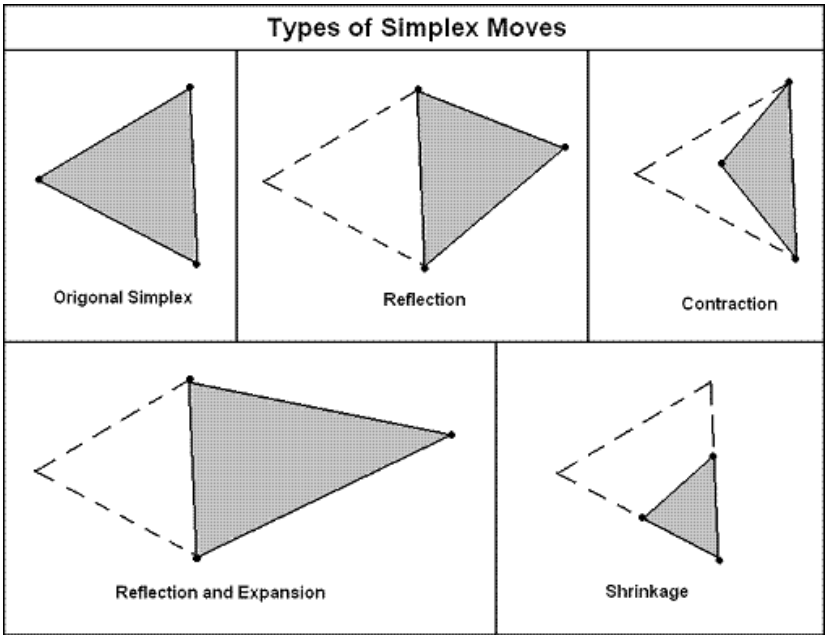
\includegraphics[width=0.5\linewidth]{./pics/ma/DownhillSimpexSchritte}
						\caption{Downhill Simplex Schritte in n = 2}
						\label{fig:DownhillSimpexSchritte}
					\end{figure}
		\subsection{\textcolor{red}{Stochastische Optimierungsverfahen}}
			\subsubsection{\textcolor{red}{Evolutionäre Algorithmen}}
				\paragraph{\textcolor{red}{Genetische Algorithmen}}
				\paragraph{\textcolor{red}{Schwarmintelligenz-Verfahren}}
	Multimodal: Funktion hat mehrere lokale Minimas.
	

	
\section{\textcolor{red}{Numerische Mathematik}}
	\subsection{\textcolor{red}{Lineare Gleichungssysteme - Lösungsverfahren}}
	\subsection{\textcolor{red}{Nichtlineare Gleichungssysteme - Lösungsverfahren}}
	\subsection{\textcolor{red}{Numerische Integration - Lösungsverfahren}}
	\subsection{\textcolor{red}{Numerische Approximation und Interpolation}}
	\subsection{\textcolor{red}{Gewöhnliche Differentialgleichungen - Lösungsverfahren}}
	\subsection{\textcolor{red}{Partielle Differentialgleichungen - Lösungsverfahren}}
	\subsection{\textcolor{red}{Eigenwertberechnung - Lösungsverfahren}}
	\subsection{\textcolor{red}{FFT - schnelle Fourier-Transformation}}

